\documentclass[10pt,final,a4paper,oneside,onecolumn]{article}

%%==========================================================================
%% Packages
%%==========================================================================
\usepackage[a4paper,left=3.5cm,right=3.5cm,top=3cm,bottom=3cm]{geometry} %% change page layout; remove for IEEE paper format
\usepackage[T1]{fontenc}                        %% output font encoding for international characters (e.g., accented)
\usepackage[cmex10]{amsmath}                    %% math typesetting; consider using the [cmex10] option
\usepackage{amssymb}                            %% special (symbol) fonts for math typesetting
\usepackage{amsthm}                             %% theorem styles
\usepackage{dsfont}                             %% double stroke roman fonts: the real numbers R: $\mathds{R}$
\usepackage{mathrsfs}                           %% formal script fonts: the Laplace transform L: $\mathscr{L}$
\usepackage[pdftex]{graphicx}                   %% graphics control; use dvips for TeXify; use pdftex for PDFTeXify
\usepackage{array}                              %% array functionality (array, tabular)
\usepackage{upgreek}                            %% upright Greek letters; add the prefix 'up', e.g. \upphi
\usepackage{stfloats}                           %% improved handling of floats
\usepackage{multirow}                           %% cells spanning multiple rows in tables
%\usepackage{subfigure}                         %% subfigures and corresponding captions (for use with IEEEconf.cls)
\usepackage{subfig}                             %% subfigures (IEEEtran.cls: set caption=false)
\usepackage{fancyhdr}                           %% page headers and footers
\usepackage[official,left]{eurosym}             %% the euro symbol; command: \euro
\usepackage{appendix}                           %% appendix layout
\usepackage{xspace}                             %% add space after macro depending on context
\usepackage{verbatim}                           %% provides the comment environment
\usepackage[dutch,USenglish]{babel}             %% language support
\usepackage{wrapfig}                            %% wrapping text around figures
\usepackage{longtable}                          %% tables spanning multiple pages
\usepackage{pgfplots}                           %% support for TikZ figures (Matlab/Python)
\pgfplotsset{compat=1.14}						%% Run in backwards compatibility mode
\usepackage[breaklinks=true,hidelinks,          %% implement hyperlinks (dvips yields minor problems with breaklinks;
bookmarksnumbered=true]{hyperref}   %% IEEEtran: set bookmarks=false)
%\usepackage[hyphenbreaks]{breakurl}            %% allow line breaks in URLs (don't use with PDFTeX)
\usepackage[final]{pdfpages}                    %% Include other pdfs
\usepackage[capitalize]{cleveref}				%% Referensing to figures, equations, etc.
\usepackage{units}								%% Appropriate behavior of units
\usepackage[utf8]{inputenc}   				 	%% utf8 support (required for biblatex)
\usepackage{csquotes}							%% Quoted texts are typeset according to rules of main language
\usepackage[style=ieee,doi=false,isbn=false,url=false,date=year,backend=biber,mincitenames=2,maxcitenames=2,mincitenames=1,uniquelist=false,uniquename=false,giveninits=true]{biblatex}
%\renewcommand*{\bibfont}{\footnotesize}		%% Use this for papers
\setlength{\biblabelsep}{\labelsep}
\bibliography{../../bib}

%%==========================================================================
%% Define reference stuff
%%==========================================================================
\crefname{figure}{Figure}{Figures}
\crefname{equation}{}{}

%%==========================================================================
%% Define header/title stuff
%%==========================================================================
\newcommand{\progressreportnumber}{16}
\renewcommand{\author}{Erwin de Gelder}
\renewcommand{\date}{March 14, 2019}
\renewcommand{\title}{Performance assessment of automated vehicles using real-world driving scenarios}

%%==========================================================================
%% Fancy headers and footers
%%==========================================================================
\pagestyle{fancy}                                       %% set page style
\fancyhf{}                                              %% clear all header & footer fields
\fancyhead[L]{Progress report \progressreportnumber}    %% define headers (LE: left field/even pages, etc.)
\fancyhead[R]{\author, \date}                           %% similar
\fancyfoot[C]{\thepage}                                 %% define footer

\begin{document}
	
\begin{center}
	\begin{tabular}{c}
		\title \\ \\
		\textbf{\huge Progress report \progressreportnumber} \\ \\
		\author \\ 
		\date
	\end{tabular}
\end{center}

\section{Previous meeting minutes}

\begin{itemize}
	\item We discussed the progress for the ontology paper. The main problem was that the literature and my own work were mixed. Therefore, it was not clear what my contribution was and what was already done in literature. 
	\item The meaning of the ``domain model'' was unclear. The ``domain model'' is a means of representing an ontology. 
\end{itemize}

\section{Summary of work}

\begin{itemize}
	\item For longer than a year, we had a plan to write a paper for the ESV conference (Enhanced Safety of Vehicles), deadline March 8. I expected that my contribution was limited as I only had to do the case study. Therefore, I never mentioned this before. It turned out that my contribution to this paper is more than only the case study, which is why I am now the first author of that paper. 
	
	In the paper with title ``a method for scenario risk quantification for automated driving systems'', we propose a method for quantifying the risk for driving scenarios, where risk is defined as the multiplication of the exposure (how frequent we encounter such a scenario) and the severity (the likelihood of a hazardous outcome when encountering such a scenario). The risk is quantified using real-world driving data.
	
	The reason that I mention this, is because I think that this paper might be a good contribution to my PhD, because quantifying the risk of particular scenarios is very useful for the performance assessment of automated vehicles. Furthermore, since real-world driving data is used to quantify the risk, the work is in line with my other work. We have some future plans (I will elaborate in a future progress report) to continue with this work. From now on, I will mention any updates regarding this work in these progress reports.
	
	FYI: The paper is attached to this report. \emph{NOTE: No review is required as the paper is already submitted.}
	
	\item The paper on the completeness is conditionally accepted for a special issue in the journal Traffic Injury Prevention. The paper needs to be submitted as a MS Word file. I converted the paper to a MS Word file. I will do a final check before submitting it (deadline is April 8). No actions from you required.
	
	\item I continued working on the paper about the ontology (attached below). Unfortunately, because the paper on risk quantification took more time, I could not finish the paper. I highlighted the changes using blue text. Few notable changes:
	\begin{itemize}
		\item Following the comment to separate literature from my own contributions, I restructured the paper:
		\begin{enumerate}
			\item Introduction
			\item Background (Why an ontology; Context of scenario; Nomenclature)
			
			\emph{This section contains knowledge from literature.}
			\item Definitions (Scenario; Event; Activity; Scenario class)
			
			\emph{This section is still a mix: it contanis the definitions of few terms and because we want the definitions to be consistent with literature, there are also many references.}
			\item Ontology (represented by a domain model)
			
			\emph{This section only contains our contributions}.
			\item Conclusion		
		\end{enumerate}
		\item I removed the term ``Activity'' from the nomenclature. First of all, no reference was made to any literature, whereas the nomenclature section should only mention definitions of terms that are directly adopted from literature. Secondly, I want to elaborate a bit more, as the activities are very important when describing a scenario. Thirdly, I want to highlight the difference between the terms ``action'' (this term is used by others, such as \textcite{ulbrich2015}) and ``activity'' and explain why we prefer the term ``activity'' (in a nutshell: activity refers to a movement \cite{caspersen1985physical}, whereas an action also includes the explanation of the movement. Therefore, actions require interpretive context \cite{bobick1997movement}).
		\item I added event to the domain model/ontology (see Fig.\ 4 of paper) and to the section on definitions (Section~III-B). Currently, the definition is similar to the definition that we had in our rejected conference paper. However, I think we need to update the definition. As can be seen in Fig.\ 4 of the paper, an event can be a trigger of an activity. Such an event could be ``the distance of the ego vehicle to the crossing becomes less than 30 meters''. Currently, however, such an event is not compliant with the definition of an event (Definition~2 of the paper).
	\end{itemize}
	\item I am following the MSc.\ course Applied Statistics (6 ECTS $\rightarrow$ 5 Graduate School (GS) Credtis).
	\item After the progress meeting, I will discuss with Mascha Toppenburg whether I can use my TNO courses to get GS credits.
	\item On March 4, a student from the Padova university (Italy) started his MSc.\ thesis at TNO. He will work on quantification of the \emph{completeness} of the data. Whereas our paper focuses on the completeness of the activities, I think the student can focus on quantifying the completeness regarding the scenario classes. A good starting point might be \cite{wang2018extracting}. In the first month, I will give the student some time to do a literature study, such that he can formulate a relevant research question for his thesis.
	\item During previous meeting, I discussed the so-called ``Milestone 3'' assessment methodology that we are developing in Singapore. The original deadline for a report on the methodology was on February 15. It appeared, however, that this was much too ambitious as the other people were very busy carrying out the ``Milestone 2'' assessment. 
\end{itemize}

\section{Future plans}

\begin{itemize}
	\item Progress with the ontology paper. Again, I plan to have a complete paper for the next meeting.
\end{itemize}

\section{Questions}

\begin{itemize}
	\item Is it a good plan to make the work on risk quantification part of my PhD thesis?
	\item Is the structure of the ontology paper OK?
	\item According to the portal of my doctoral education, the Go/No Go meeting is not yet completed. I think action point lies at Bart.
\end{itemize}


\printbibliography


\newpage
\includepdf[pages=-,pagecommand={},width=\paperwidth]{../../"20180639 Journal paper ontology"/journal_ontology.pdf}
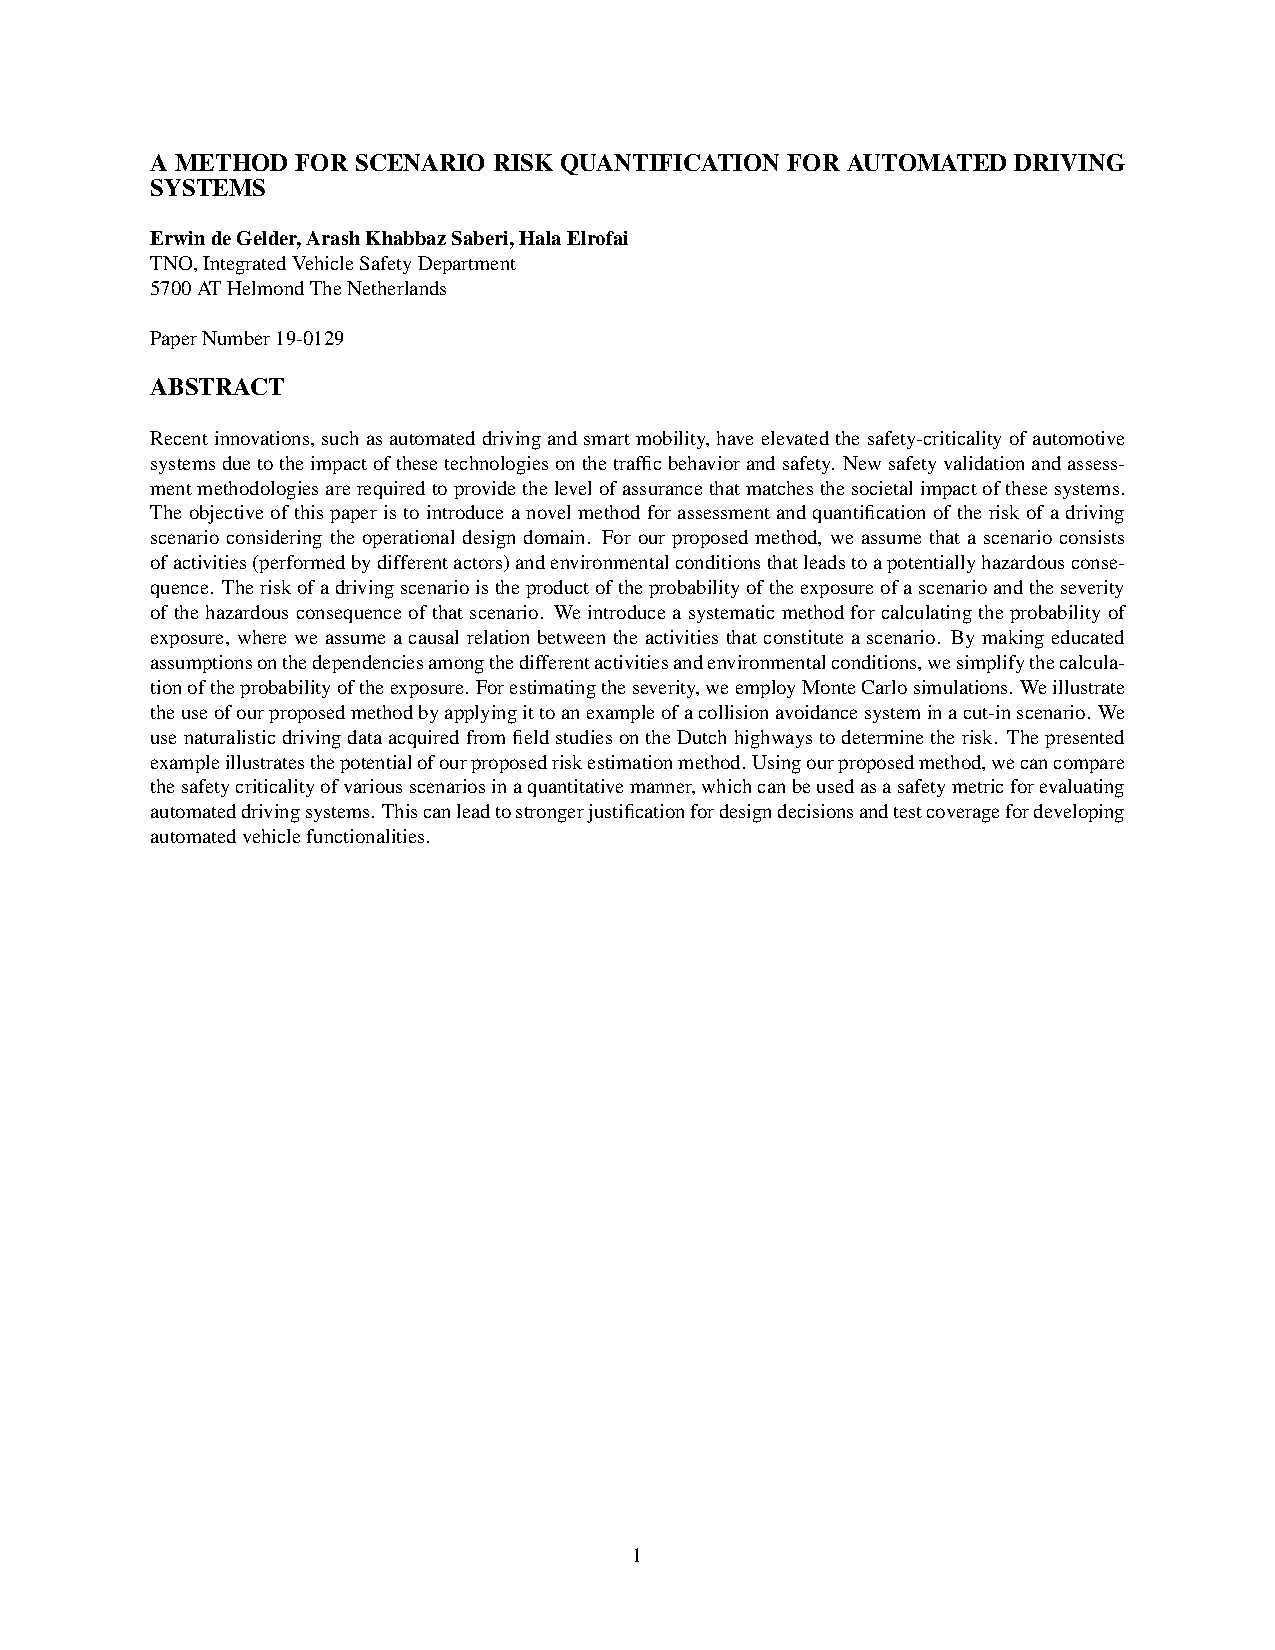
\includepdf[pages=-,pagecommand={},width=\paperwidth]{RiskPaper_ESV2019-Format.pdf}


\end{document}